\section{Theoretical Background}

\subsection{Wave channel}

A wave channel is a water tank that provides a small environment to reproduce phenomena occurring on the coast or in the open sea. Its size and shape vary by usage, from small rectangular tanks to long and wide square tanks. The one at the lab is a length of $6,000\mathrm{~mm}$, a width of $300\mathrm{~mm}$, and a height of $400\mathrm{~mm}$: It was extended during the research. The 3-dimensional wave channel is widely used for its broad spectrum of waves generated. The 3-dimensional means that the wave could be generated with vortexes: the fluid is rotational($\nabla \times \vec{v} \neq 0$). On the other hand, a 2-dimensional wave channel can only be used for generating waves without vortexes: the wave channel is usually rectangular and the waves progress along the side, without perpendicular fluid movement.

Previously, a small rectangular parallelepiped wave channel with a dimension of length $4,000\mathrm{~mm}$, a width of $300\mathrm{~mm}$, and a height of $400\mathrm{~mm}$ was built and utilized in the lab. It is constituted of 2 modules, each with a length of $2,000\mathrm{~mm}$, and they were connected and sealed to prevent water leakage. The frame is made of an aluminum profile and the walls are made of transparent acrylic plates $5\mathrm{~mm}$ thickness. Also, there are wheels at the bottom for mobility, height adjustment, and horizontal adjustment. It was mainly built to test the masonry structure of breakwater, but it could be used to test the stability of a ship or the durability of a coastal structure, providing an appropriate environment.

\subsection{Wavemaker}

A wavemaker is a device that generates waves in a wave channel. It is usually categorized by the movement of the plate. In general, there are piston types, plunger types, flap types, etc \cite{Edinburgh_Designs_Ltd_2016}.

\begin{figure}[H]
    \begin{center}
        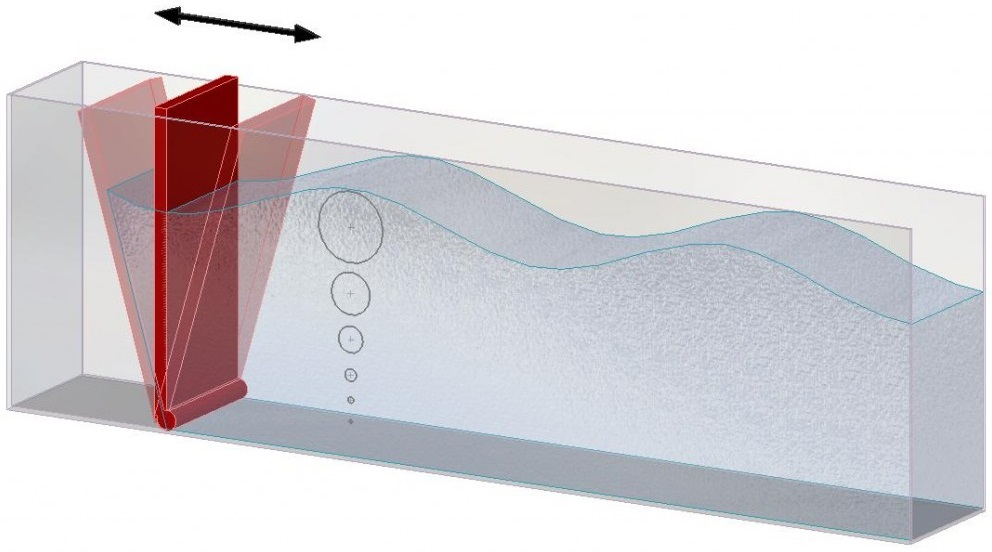
\includegraphics[height=3cm]{images/Wave_Maker(Flap).jpg}
        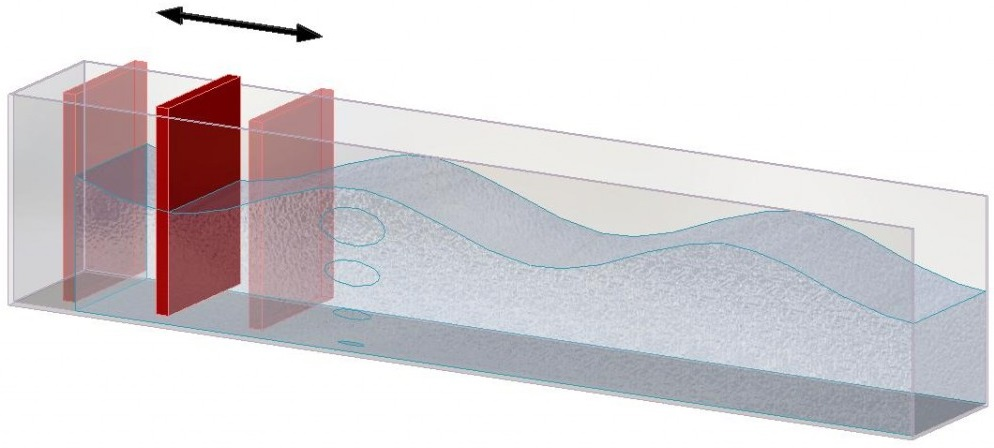
\includegraphics[height=3cm]{images/Wave_Maker(Piston).jpg}
    \end{center}
        \begin{tikzpicture} [remember picture, overlay]
            \node at (1.7, 1.0) {\scriptsize{(a) flap type}};
            \node at (7.6, 1.0) {\scriptsize{(b) piston type}};
        \end{tikzpicture}
        \caption{Various types of 2-dimensional wavemaker - (a) flap type (b) piston type}
        \label{Experimnet_System} 
\end{figure}

A piston-type wavemaker was built for the research, with the plate moving horizontally to push water. It can only generate 2-Dimensional waves, progressing in one direction; In fact, various types of waves (especially 3-Dimensional) can be generated if the plate has steps, each part moving in a certain sequence (It is called snake-like). Theoretically, the plate should move sinusoidally to generate sinusoidal waves. There is a range that the plate moves within, and it is called Stroke, denoted as $S_0$ hereinafter.

Previously, a small wavemaker was built for the former study, using a linear actuator of length 40$\mathrm{cm}$. It's a piston type, with an acrylic plate designed to fit in the wave channel. Both actuators and motor drivers utilize products of FUYU, Chengdu, but the wavemaker has the limitation of not being able to generate various waves. There is a controller, but it only changes the wave in several versions, without proper parameters that intermediate the generation of wave theoretically. To experiment successfully with models, certain conditions should be satisfied, based on model experiment principles such as Froude's law or Reynolds' law \cite{briggs2013basics, chakrabarti1994offshore}.

\subsection{Wavemaker theory}

Wavemaker theory investigates the properties and shapes of waves generated by the motion of the wavemaker within the wave channel. Fluids inside the tides must satisfy several principles of hydrodynamics and boundary conditions \cite{dean1991water, zhang2007deterministic}. Few differential equations and boundary conditions are derived from the geometry of the wave channel and the basic principle. The solution is the velocity potential, which gives the shape of the wave, its velocity, and other physical variables. It is expressed as a wave packet: the sum(superposition) of infinite waves of different wave numbers. The goal of the theory is to find out the relationship between the wave's shape and the plate's movement under the assumption that the plate moves sinusoidally.

\begin{figure}[h]
    \centering
    \captionsetup{}
    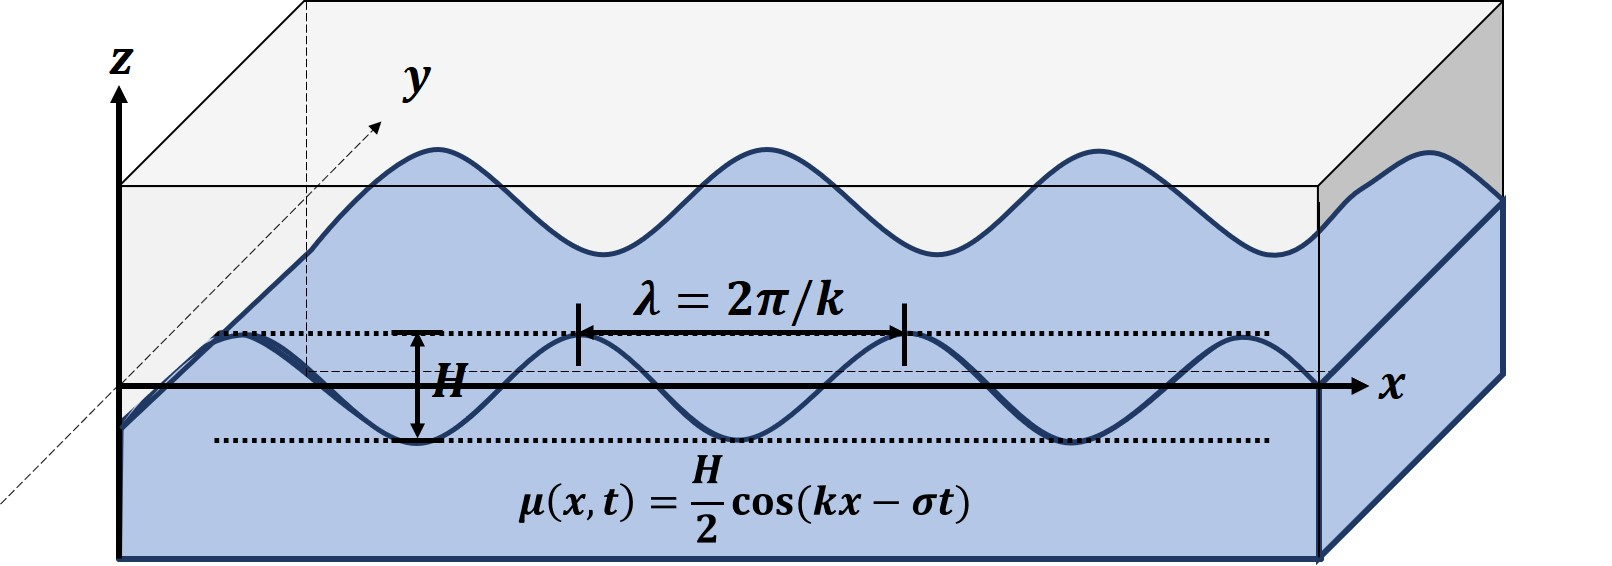
\includegraphics[width=13cm]{images/Water_Channel(Illustrated).jpg}
    \caption{Illustration of the wave channel}
    \label{Water_tank(Illustrated)}
\end{figure}

Several references start by inducing the Laplace equation about velocity potential. Before that, it should be guaranteed that the velocity potential can be defined. Let's begin with the continuity equation of mass. The Lagrangian differential for density $\rho$ is zero because the mass is conserved regardless of the type of fluid.
%
\begin{equation}
    {D\rho/Dt = d\rho/dt + \Vec{v} \cdot \nabla\rho = 0}\label{eq_001}
\end{equation}

$\rho$ is constant when the fluid is incompressible. Often, water is assumed to be incompressible, and it's not a major focus of the theory and experiment.

\begin{equation}
    {d\rho/dt = 0,~\nabla \cdot \vec{v} = 0}\label{eq_002}
\end{equation}

In a 2-Dimensional wave channel, fluid is irrotational: the curl of $\vec{v}$ is zero.
\begin{equation}
    {\nabla \times \vec{v} = 0}\label{eq_004}
\end{equation}

As a result, the potential function of the velocity field $\phi(x, z, t)$ can be defined and it satisfies the Laplace equation.

\begin{equation}
    \vec{v} = - \nabla \phi, ~\nabla^2 \phi = 
    \frac{\partial^2 \phi}{\partial x^2} + 
    \frac{\partial^2 \phi}{\partial z^2}\label{eq_005}
\end{equation}

$\phi(x, z, t)$ is a solution that meets several boundary conditions. By Kinematic Free-Surface boundary condition (denoted as KFSBC hereinafter), the shape of the free surface (water-air interface) $\eta(x, t)$ is expressed as:

\begin{equation}
    \eta = \frac{1}{g} \frac{\partial \phi}{\partial t}|_{z=0}\label{eq_007}
\end{equation}

Since $\eta$ is a displacement, it is related to $\phi$ by $v_{z}$ of the wave.
\begin{equation}
    -\frac{\partial \phi}{\partial z}|_{z=0} = \frac{\partial \eta}{\partial t}|_{z=0}\label{eq_008}
\end{equation}

$\eta$ is the shape of the wave, one of the main goals of wavemaker theory. Also, there are horizontal and vertical geometric boundary conditions:

\begin{enumerate}
    \item Vertically, the z-directional velocity at the bottom of the channel($z=-h$) should be zero.
    \begin{equation}
        \frac{\partial \phi}{\partial z}|_{z=-h} = 0\label{eq_009}
    \end{equation}

    \item Horizontally, there is a plate at one end of the channel. Denote the displacement of the plate as $S(z)$ (it is x-directional), and the boundary condition is expressed as:
    \begin{equation}
        F(x, ~z, ~t) = x - \frac{S(z)}{2} \sin{\sigma t} = 0\label{eq_010}
    \end{equation}

    This is one type of Kinematic boundary condition, and it must satisfy ${DF/Dt} = 0$. This condition can differ by the motion of the plate. The \textit{signal} for the wave plays its role here.
    \begin{equation}
        \frac{\partial F}{\partial t} = {\vec{v} \cdot \nabla F}\label{eq_011}
    \end{equation}

    \begin{equation}
        u - \frac{w}{2}\frac{\partial S}{\partial z}\sin{\sigma t} = \frac{S(z)}{2} \sigma \cos{\sigma t}\label{eq_012}
    \end{equation}

    With Taylor expansion, the boundary condition is derived by Taylor expanding Equation \ref{eq_012} at $x=0$.
    
    \begin{equation}
        u(0, ~z, ~t) = \frac{S(z)}{2} \sigma \cos{\sigma t} \label{eq_013}
    \end{equation}
    
\end{enumerate}

Solving Equation \ref{eq_005} with boundary condition, the solution is as follows:
\begin{equation}
    \phi(x, ~z, ~t) = A_p \cosh{k_p (h+z)} \sin{(k_p x - \sigma t)} + (Ax + B) + C \exp(-k_p x) \cos{k_s (h+z)} \cos{\sigma t}\label{eq_014}
\end{equation}

The first term represents the progressive wave, whereas the second term represents the free stream, which is generally zero. The third term represents a standing wave, with its amplitude decreasing exponentially. Especially, $k_s$ is the solution of the dispersion relation, which exists infinitely many.

Changing the form of Equation \ref{eq_008}:
\begin{equation}
    \frac{\partial \phi}{\partial z}|_{z=0} - \frac{\sigma^2 \phi}{g}|_{z=0} = 0\label{eq_015}
\end{equation}

\emph{Dispersion Relation}:
\begin{equation}
    \sigma^2 = gk_{p} \tanh{k_p h}\label{eq_016}
\end{equation}

Substituting Equation \ref{eq_016} with standing wave number $k_s$ gives:
\begin{equation}
    \sigma^2 = -gk_{s} \tan{k_s h}\label{eq_017}
\end{equation}

There are infinitely many solutions of Equation \ref{eq_017}, and let's denote the positive solution in the increasing order as $k_{s}(n)$: $k_{s}(1)$, $k_{s}(2)$, $k_{s}(3)$, ...\\
Expressing Equation \ref{eq_014} with linear combination with $k_{s}(n)$ as coefficients:
\begin{equation}
    \phi(x, ~z, ~t) = A_p \cosh{k_p (h+z)} \sin{(k_p x - \sigma t)} + \sum_{n=1}^{\infty} C_{n} \exp(-k_{s}(n) x) \cos{k_{s}(n) (h+z)} \cos{\sigma t}\label{eq_018}
\end{equation}

Again, the first term represents the progressive wave and the second term(linear combination) represents the standing wave decreasing exponentially. $k_s (n)$ is related to the damping coefficient of Equation \ref{eq_018} and the first mode has the smallest effect toward damping by $x$. Numerically, $k_s (1)$ exists between $\pi/2$ and $\pi$, and the amplitude of the mode decreases by the proportion of $exp(-k_s (1) x)$: 0.04 when $x=2h$, 0.009 when $x=3h$. For a long wave channel, the amplitude rapidly decreases. The length of the wave channel is $6m$ with water depth lower than $30cm$, which gives $x>20h$: The standing wave might be negligible.

Equation \ref{eq_018} must satisfy boundary condition - Equation \ref{eq_013}:
\begin{equation}
    u(0, ~z, ~t) = \frac{S(z)}{2} \sigma \cos{\sigma t} = - \frac{\partial \phi}{\partial x}|_{x=0}\label{eq_019}
\end{equation}
\begin{equation}
    \frac{S(z)}{2} \sigma = - A_p k_p \cosh{k_p (h+z)} + \sum_{n=1}^{\infty} C_n k_s (n) \cos{k_s (n) (h+z)}\label{eq_020}
\end{equation}

In the case of the research, $S(z)$ is constant: $S(z) = S_0$. It's the simplest form of \textit{Piston type Wavemaker}. Also, coefficients from Equation \ref{eq_020} can be derived from orthogonality. With all this information, the shape of the wave is:
\begin{equation}
    \eta(x, t) = \frac{A_p \sigma}{g}\cosh{k_p h} \cos{(k_p x - \sigma t)} + \sin{\sigma t} \sum_{n=1}^{\infty} \frac{\sigma C_n}{g} \exp{(-k_s (n) x)} \cos{(k_s (n) h)}
    \label{eq_021}
\end{equation}

Similar to Equation \ref{eq_014} and Equation \ref{eq_018}, the first term represents a progressive wave and the second term represents standing waves, decreasing exponentially. As discussed earlier, the standing waves are negligible and the wave height $H$ can be expressed by linearly approximating each eigenfunction.
\begin{equation}
        H = \frac{4 S_0 \sinh{kh}}{\sinh{2kh} + 2kh}(\sinh{k(z_d - h)} - \sinh{k(z_u - h)})\label{eq_022}
\end{equation}

From Equation \ref{eq_022}, $k$ is the wave number formerly given($k_p$), and $z_u$, $z_d$ denotes the depth of the plate, each corresponding to the upper part and the bottom part, respectively. If the plate exists throughout the depth, $S(z) = S_0$, $z_d = h$, and $z_u = 0$. Wave height and the wave function are expressed as:
\begin{equation}
    \eta(x, ~t) = \frac{H}{2} \cos{(kx-\sigma t)}, ~H = \frac{4 S_0 \sinh^2 {kh}}{\sinh{2kh} + 2kh} = \frac{4 S_0 \sinh^2 {z}}{\sinh{2z} + 2z}~(z=kh)
    \label{eq_023}
\end{equation}

From Equation \ref{eq_023}, several numbers such as \emph{Stroke} $S_0$ and depth of the water $h$ can be regulated externally. Also, wave number $k$ and angular frequency $\omega$ are related by dispersion relation (Equation \ref{eq_016}), so only $k$ or $\omega$ is needed to be set with proper structural conditions.

This theory has been expanded with a lot of approximations of boundary conditions and calculations. $H/h$ and $H/\lambda$ should be small enough for it, and on other occasions, nonlinear theories like Stokes Nonlinear Wave Theory and Cnoidal Wave Theory are needed. In a special case, a tsunami is generated by Solitary Wave Theory \cite{madsen1970waves, watts1998wavemaker, fenton1990nonlinear}.

\subsection{Wave absorber}

As the wave is generated by the wavemaker, it progresses inside the tank and is divided into progressive waves and reflected waves reflected by the surrounding obstacles, such as walls or other coastal models. According to the principle of superposition, the surface wave is expressed as a linear combination of the progressive wave and the normal wave by reflection, and the normal wave is the main cause of the error from an experiment. A wave absorber is a device that prevents or extinguishes these reflected waves: Generally, they are divided into active and passive types \cite{ouellet1986survey}.

The active absorber is another wavemaker, but it should generate a new wave to completely offset the incident wave. It requires abilities to measure the incident wave and generate the proper wave immediately, by moving the plate. It is fairly expensive equipment and has limited use since it is designed to use in specific environments. This method is to install another wavemaker near the wall where the incident wave collides, and the wavemaker controls its motion to generate the wave that offsets the reflected wave. This is called the "Absorbing Wavemaker", and it should be possible to measure the shape of the wave by the plate and to perform overlapping motion accordingly \cite{frigaard1995absorbing}. The reflection coefficient can be significantly reduced, but its usability is not as wide as a passive wave absorber.

The passive wave absorber aims to minimize the energy of the reflected wave by installing an additional structure. Unlike active absorbers, it is impossible to completely extinguish reflective waves for passive ones, no matter how optimized they are. Also, there are various structures such as horsehair, crushed rock, etc. In particular, porous structures are used to effectively extinguish waves, and many studies have been conducted on it, such as a comparison of reflection coefficients according to porosity, and their efficiency has already been proven. In addition, ramps are also used to minimize reflective waves in 3-Dimensional waves, in areas that researchers are not interested in. It was found that the convex parabolic surface had the lowest reflection coefficient.

\subsection{Froude Similarity Law}

Physical features change as the dimension of the physical system changes. The scale factor between the real system and the experimental model is needed, and the Froude Similarity Law is held \cite{briggs2013basics, chakrabarti1994offshore}.
\begin{equation}
    Fr_{1} = Fr_{2}, ~Fr = \frac{V}{\sqrt{gL}}
    \label{froude number}
\end{equation}

$V$ is the velocity of the moving element, $L$ is the characteristic length of the system, and $g$ is the gravitational acceleration. There are other dimensionless numbers such as the Prantdl number, Reynolds number, etc. but the gravitational effect is dominant rather than the viscosity of the fluid or diffusion.

The moving element of both systems 1 and 2 (which is wave channel and open sea, respectively) is water(wave), so the Froude number is expressed as equation \ref{froude number of wave} with a dispersion relation.

\begin{equation}
    Fr_i = \sqrt{\frac{\tanh{k_i h_i}}{k_i L_i}}
    \label{froude number of wave}
\end{equation}

\begin{enumerate}
    \item System1: Wave Channel
    
    It is known that the characteristic length of the channel with a rectangular cross-section is $L_2 = \frac{2ah_1}{a+h_1}$, where $a$ and $h_1$ correspond to the width and depth of the channel, respectively.
    \begin{equation}
        Fr_1 = \sqrt{\frac{\tanh{k_1 h_1}}{k_1 h_1} \times \frac{a+h_1}{2a}}
    \end{equation}
    
    \item System2: Open Sea
    
    There are no references to the characteristic length of the open sea. It's assumed that the open sea is a large rectangular channel with $h_2 \gg\ a$, which gives $L_{2} = 2h_{2}$, where $h_2$ is the depth of the water.
    \begin{equation}
        Fr_2 = \sqrt{\frac{\tanh{k_2 h_2}}{k_2 h_2} \times \frac{1}{2}}
    \end{equation}
\end{enumerate}

Froude numbers of both systems agree:
\begin{equation}
    \frac{a+h_1}{2a} f(z_{1})  = f(z_{2})
    \label{froude number equation}
\end{equation}

where $f(x) = \frac{\tanh{x}}{x}$ and $z_i = k_i h_i$. The experiment condition was set as $a = 0.30m$, $h_{1} = 0.15m$. Also, the wave is categorized by $h/\lambda < 1/20$ (long wave) and $h/\lambda > 1/2$ (short wave). With these constants, Equation \ref{froude number equation} gives numerical solutions: $\omega \sim \pi$ for the long wave and $\omega \sim 4\pi$ for the short wave. In the case of a sinusoidal wave, $\omega \sim 4\pi$.

%%%%%%%%%%%%%%%%%%%%%%%%%%%%%%%%%%%%%%%%%%%%%%%%%%%%%%%%%%%
% \section{Theoretical Background}

% \subsection{Wave Channel}

% A wave channel is a tank that creates a small environment to reproduce phenomena occurring on the coast or in the open sea. Its size and shape vary by usage, from small rectangular tanks to long and wide square tanks. The one at the school has a length of 6,m, a width of 30, cm, and a height of 40, cm. The 3-Dimensional wave tank is the most popular since it's suitable for using a wave maker that generates 3-Dimensional waves. The "3-Dimensional" means that the wave is generated with vortexes: the fluid is rotational ($\nabla \times \vec{v} \neq 0$). On the other hand, "2-Dimensional" means that the wave is generated without vortexes: if the wave channel is rectangular and the waves progress along the side, there is no perpendicular fluid movement.

% Previously, a small rectangular parallelepiped wave tank with dimensions of length 6,m, width 30, cm, and height 40, cm was built and utilized. It is constituted of 2 modules, each with a length of 2,m, and they were connected and sealed to prevent water leakage. The frame is made of aluminum profile, and the walls are made of transparent acrylic plates (5, T: 5, mm thick). Also, there are wheels at the bottom for mobility, height adjustment, and horizontal adjustment. It was mainly built to test the Masonry structure of breakwater, but it could be used to test the stability of a ship or the durability of a coastal structure, providing an appropriate environment.

% \subsection{Wave Maker}

% A wave maker is a device that generates waves in a wave channel. It is usually categorized by the movement of the plate. In general, there are piston types, plunger types, flap types, etc.

% \begin{figure}[H]
% \centering
% \captionsetup{justification=centering}
% 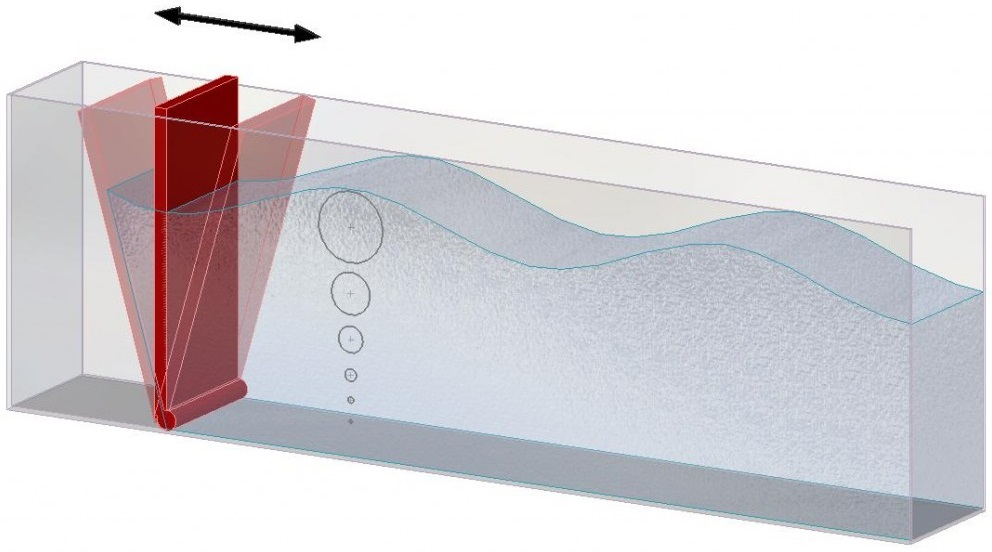
\includegraphics[height=3cm]{images/Wave_Maker(Flap).jpg}
% 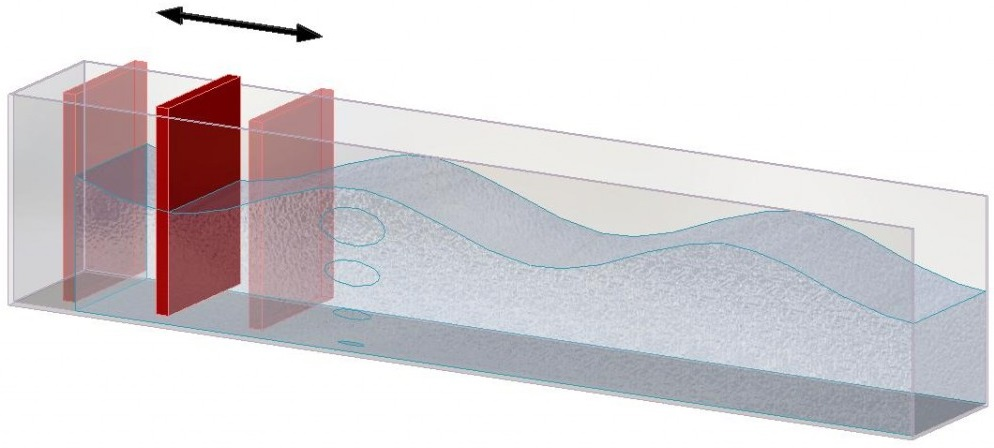
\includegraphics[height=3cm]{images/Wave_Maker(Piston).jpg}
% \caption{Flap type (left) and Piston type (right) wave maker}
% \label{various types of wave makers}
% \end{figure}

% A piston type was built for this research, with each element (part) of the plate moving horizontally to push water. The plate is not separated by each part: it moves as a single, integrated body. It can only generate 2-Dimensional waves, progressing in one direction. Various types of waves (especially 3-Dimensional) can be generated if the plate has steps, and each part moves in a certain sequence (referred to as \textit{snake-like}). Theoretically, the plate should move sinusoidally to generate sinusoidal waves. There is a range that the plate moves within, and it is called \textit{Stroke}, denoted as $S_0$ hereinafter.

% Previously, a small wave maker was built for the former study, using a 40, cm long linear actuator. It is a piston type, with an acrylic plate that is designed to fit the size of the tank. Both actuators and motor drivers utilize products of \textit{FUYU, Chengdu}, but the wave maker has the disadvantage of not being able to generate various waves. There is a controller, but it only changes the wave in several versions, without proper parameters that intermediate the generation of waves. It cannot control the phase velocity or wave height. Therefore, the wave generator for this research needs to be improved.

% \subsection{Wave Parameters}

% There are various parameters used to describe waves. Some of the important ones are:

% \begin{itemize}
% \item Wave Height ($H$): The vertical distance between the crest and trough of a wave.
% \item Wave Length ($L$): The horizontal distance between two successive crests or troughs of a wave.
% \item Wave Period ($T$): The time taken for a wave crest to travel a distance equal to one wavelength.
% \item Wave Number ($k$): The spatial frequency of the wave, defined as $k = \frac{2\pi}{L}$.
% \item Phase Velocity ($C$): The speed at which a specific phase of the wave (e.g., crest) moves in a particular direction.
% \item Group Velocity ($C_g$): The speed at which the energy of a wave group (composed of multiple waves) propagates.
% \end{itemize}

% These parameters play a crucial role in characterizing the behavior and properties of waves.

% \subsection{Wave Absorption}

% In a wave channel, wave absorption is necessary to prevent the reflection of waves from the boundaries of the tank, which could interfere with the desired wave patterns. Different techniques can be employed for wave absorption, such as:

% \begin{itemize}
% \item Sloping Beach: The tank bottom is inclined towards the wave-maker end, allowing the waves to dissipate their energy as they reach the boundary.
% \item Porous Structures: Placing porous materials at the tank boundaries to absorb and dissipate the energy of the waves.
% \item Wave Dissipators: Installing specialized structures, such as perforated plates or wave absorbers, to dampen the wave energy and prevent reflection.
% \end{itemize}

% The choice of wave absorption technique depends on the specific requirements of the experiment or simulation being conducted in the wave channel.

% \subsection{Wave Measurement}

% To analyze and study wave behavior in the wave channel, various measurement techniques can be employed, including:

% \begin{itemize}
% \item Wave Gauges: Sensors placed in the tank to measure the water surface elevation and obtain wave height and wave period data.
% \item Laser Doppler Vibrometry: Using laser beams to measure the velocity of the water particles and obtain information about wave characteristics.
% \item Video Analysis: Recording videos of the waves and analyzing them using image processing techniques to extract wave parameters.
% \end{itemize}

% These measurement techniques enable researchers to gather quantitative data about the waves generated in the wave channel.

% In conclusion, the wave channel and wave maker provide a controlled environment for studying wave phenomena. Understanding wave parameters, absorption techniques, and measurement methods is crucial for conducting accurate experiments and simulations in the wave channel.

